% Font size, paper type
\documentclass[12pt]{article}
% Aesthetic margins
\usepackage[margin=1in]{geometry}
% Core math packages,
% Mathtools loads amsmath, and amsmath gives basic math symbs
% Amsfonts & amssymb are misc. symbols you might need
\usepackage{mathtools, amsfonts, amssymb}
% Links in a pdf
\usepackage{hyperref}
% Use in pictures, graphs, and figures
\usepackage{graphicx}
% Header package
\usepackage{fancyhdr}
% Underlining with line breaks
\usepackage{ulem}
% Adjust accordingly given warning messages
\setlength{\headheight}{15pt}
% So we can more easily format text with pictures
\usepackage{float}
% Images and drawing graphs
\usepackage{tikz}

% Sets footer
\pagestyle{fancy}
% Removes default footer style
\fancyhf{}

\rhead{
  Shengdong Li
  Calc 3
}

\rfoot{
  Page \thepage{}
}

% Makes links look more appealing
\hypersetup{
    colorlinks=true,
    linkcolor=cyan,
    filecolor=magenta,      
    urlcolor=cyan,
}

% \usepackage{indentfirst}

\begin{document}
\title{Lab 3 Eggdrop}
\author{by Shengdong Li}
\date{23 February 2021}
\maketitle

\tableofcontents
\bigskip

\textbf{Purpose:} In this lab, you and your team of BOGmates will use your knowledge of physics in two dimensions to drop an egg on your instructor.

\section{Monday}

\textbf{Given:} Your instructor will walk at constant velocity beneath the announcer’s booth of the varsity baseball field (a two-story tower).  Your in-person teammate of choice will stand tall on top of the announcer booths’ steps, with her or his dropping hand raised above her/his head.  The egg must freefall to strike the helmet of the instructor (you may not throw the egg down).

\subsection{Team}
\begin{itemize}
	\item{1 egg dropper}
	\item{1 assistant to dropper, making measurements}
	\item{1 camera person, data collector/relayer/communicator to BOGmates (must have a modern phone with video camera and data connection, and will post team’s video to web and send link to all teammates)}
	\item{1 at-home leader who will communicate with in-person communicator (must have a sell phone)}
	\item{
	      Remainder collaborate and seek consensus on all calculations, and communicate clear instructions remotely  to in-person teammates
	      }
\end{itemize}

Link to teammate spreadsheet for \href{https://docs.google.com/spreadsheets/d/112zGZxcq4Y2s_ZFFPWRVIT6ZBOVhoSKDDAyddDDMR_E/edit#gid=1855240678}{period 2}

\section{Friday}

Identify and describe what variables / information you will need to know before the drop

\subsection{Mode of communication}

We will communicate with each other using a shared Google doc

\subsection{Equations of motion, and variables}

\begin{align*}
	\intertext{The total height of egg and dropper}
	h_{egg}       & =h_{platform}+h_{dropper} \\
	\intertext{The total height of Mr. Schilling with a helmet}
	h_{schilling} & =1.89m                    \\
	\intertext{The total height of the dropper with hand raised}
	h_{dropper}   & =?                        \\
	\intertext{The total height of the platform}
	h_{platform}  & =?                        \\
	\intertext{The total height that the egg will drop}
	h_{drop}      & =h_{egg}-h_{schilling}    \\
	a             & =9.80\frac{m}{s^2}        \\
	\intertext{Mr. Schilling's constant velocity}
	v_{schilling} & =?                        \\
	\intertext{The equation for displacement given a constant velocity and acceleration}
	x             & =v_{0}t+0.5at^{2}         \\
	\intertext{The equation for displacement given a velocity and time}
	x             & =vt                       \\
	\intertext{The equation for velocity given velocity and time}
	v             & =\frac{x}{t}              \\
\end{align*}


\subsection{Materials}

\begin{itemize}
	\item{1 safety helment}
	\item{1 measuring tape}
	\item{1 actual tape}
	\item{1 egg}
\end{itemize}

\subsection{When dropper will drop}

\begin{align*}
	\intertext{First calculate the time \(t\) it takes for egg to drop, where \(a\) = \(9.8 \frac{m}{s^2}\)}
	t          & =\sqrt{\frac{2\left(h_{egg}-h_{schilling}\right)}{a}} \\
	\intertext{Next calculate the distance that \(x\) that Mr. Schilling will move in the time that it takes for the egg to drop  }
	x          & =vt                                                   \\
	\intertext{Finally, subtract the total distance away from the distance that Mr. Schilling will move}
	d_{away}-x & =d_{tape}                                             \\
	\intertext{Tape the measured point. When Mr. Schilling moves over that piece of tape, let the dropper release the egg!}
\end{align*}
Tape the measured point. When Mr. Schilling moves over that piece of tape, let the dropper release the egg!

\section{Lab Report}

\textbf{Include all of the above, along with the following}

\subsection{Procedure + Sketch}
Describe your team's process for this lab \ldots what was your strategy?

\subsubsection{How fast is Mr. Schilling}

\begin{figure}[H]
	\begin{center}
		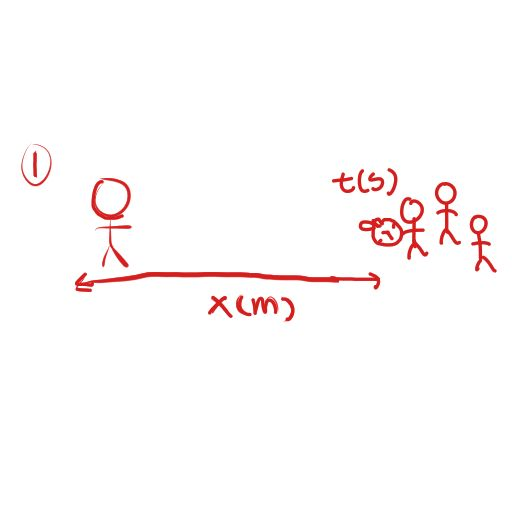
\includegraphics[scale=2]{1.JPEG}
	\end{center}
\end{figure}

\begin{align*}
	\intertext{To calculate Mr. Schilling's speed, we must find out how far Mr. Schillling will walk}
	x         & =?            \\
	\intertext{During the walk, we need to time how long it takes for the walk to complete}
	t         & =?            \\
	\intertext{With these two variables, we can then calculate the average velocity,}
	\Aboxed{v & =\frac{x}{t}}
\end{align*}

\subsubsection{Time it takes for egg to drop}

\begin{figure}[H]
	\begin{center}
		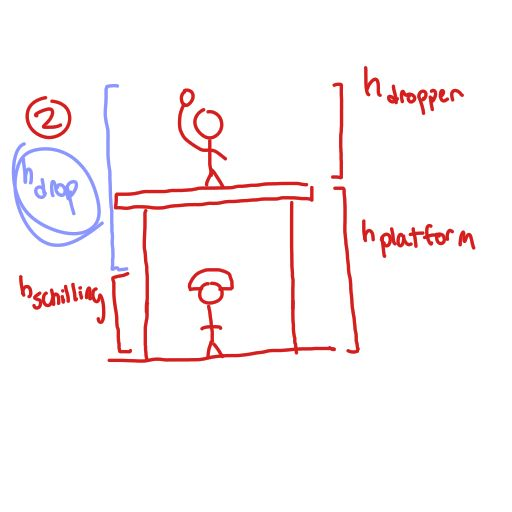
\includegraphics[scale=2]{2.JPEG}
	\end{center}
\end{figure}

\begin{align*}
	\intertext{To calculate the amount of time it takes for the egg to drop, we must first calculate how far the egg will fall. }
	\intertext{Recall that Mr. Schillling's height is }
	h_{schilling} & =1.89m                                   \\
	\intertext{Next measure the droppers height}
	h_{dropper}   & =?                                       \\
	\intertext{Next measure the height of the platform}
	h_{platform}  & =?                                       \\
	\intertext{The total height that the egg drops is subtracted by Mr. Schilling's height}
	x             & =h_{dropper}+h_{platform}-h_{schilling}  \\
	\intertext{To calculate how long it takes the egg to fall, we will use the equation}
	x             & =v_{0}t+\frac{1}{2}at^{2}                \\
	\intertext{And solve for \(t\)}
	t             & =\sqrt{\frac{2\left(x-v_{0}t\right)}{a}} \\
	\intertext{However, we know that we're dropping the egg from rest, so we can set that to 0, and we know the acceleration of gravity}
	\Aboxed{t     & =\sqrt{\frac{2x}{9.80\frac{m}{s^{2}}}}}  \\
\end{align*}



\subsubsection{When to drop the egg}

\begin{figure}[H]
	\begin{center}
		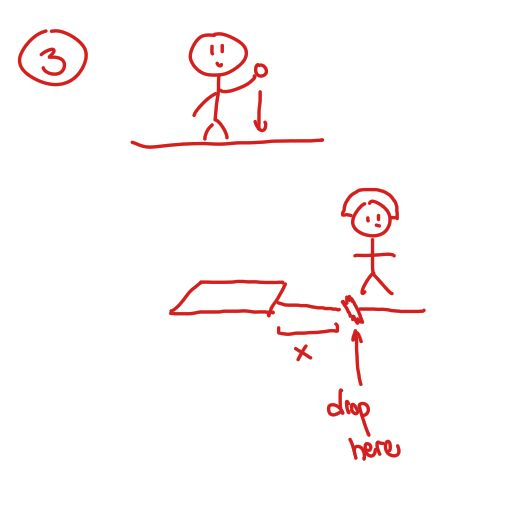
\includegraphics[scale=2]{3.JPEG}
	\end{center}
\end{figure}

\begin{align*}
	\intertext{To calculate when to drop the egg, we'll multiply our previous value of time it takes for egg to drop by Mr. Schilling's average velocity}
	\Aboxed{x & =vt}
	\intertext{Then we mark off from the left with some same where we will drop. After Mr. Schilling walks over the piece of tape we will drop the egg immediately}
\end{align*}

\subsection{Analysis}
Include all calculations, showing your work and reasoning. Describe your results (did you hit me or not? How close? Did the egg hit in front of me, behind me, or wherre? What would you do differently next time?)

\begin{align*}
	\intertext{Mr. Schilling's average velocity}
	x & =\frac{dx}{dt}                          \\
	d & =1                                      \\
	t & =1                                      \\
	  & =\frac{20.0m-0m}{9.74s-0s}              \\
	  & =2.05\frac{m}{s}                        \\
	\intertext{Height of drop}
	x & =h_{platform}+h_{dropper}-h_{schilling} \\
	  & =\left(2.06m+2.88m\right)-1.89m         \\
	  & =3.05m                                  \\
	\intertext{How much will Mr. Schilling walk in that time}
	x & =vt                                     \\
	  & =0.79s\cdot2.05\frac{m}{s}              \\
	\intertext{The final distance that we would mark with tape from the paper would be}
	  & =\boxed{1.6195m}                        \\
\end{align*}

\subsection{Conclusion}

The calculations done to arrive at the distance of \(1.6195m\) where we should mark with tape and drop the egg all seemed to be correct. However, in the end, our egg landed a few inches behind Mr. Schilling without hitting the safety helment.

\subsubsection{Error}

This was a close result, but the error could've been due to a variety of reasons. One factor that we did not account for was air resistance. Because there was some air resistance in the atmosphere, the egg was not in a true freefall, and it could have slowed the egg down by a miniscule amount, causing it to fall slower and thus land behind Mr. Schilling. Other errors could be human error: The time in which Joshua actually saw Mr. Schilling cross the tape vs. when Joshua dropped the egg could've caused slight error. Having only gotten an average of 3 trials where Mr. Schilling walked along the path could've also caused some error.

\subsection{Future}

In the future, were we to do this experiment again, we would make sure to get more trials on Mr. Schilling's walks to better calculate his average velocity. If we could, we would also practice dropping the egg to minimize hand-eye coordination error. Finally, we throw the egg down a vacuum chamber to minimize the effects of air resistance.
\end{document}